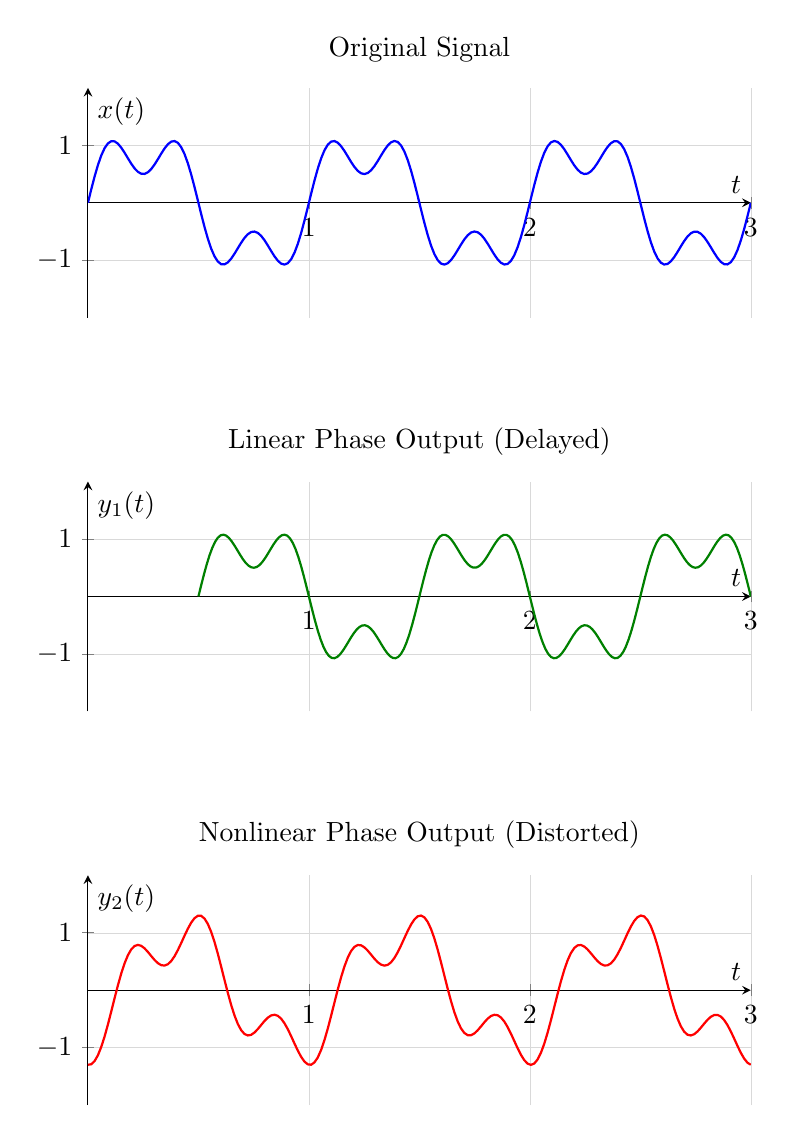
\begin{tikzpicture}
	% Define a common style
	\pgfplotsset{
		phase b/.style={
			width=10cm, height=4.5cm,
			axis lines=middle, xlabel={$t$},
			xmin=0, xmax=3, ymin=-2, ymax=2,
			xtick={1,2,3}, ytick={-1,1},
			grid=major, grid style={line width=.1pt, draw=gray!30},
			no marks,
			samples=200,
		}
	}
	\begin{scope}[yshift=10cm]
		\begin{axis}[phase b, title={Original Signal}, ylabel={$x(t)$}]
			\addplot[blue, thick, domain=0:3] {sin(deg(2*pi*x)) + 0.5*sin(deg(6*pi*x))};
		\end{axis}
	\end{scope}
	\begin{scope}[yshift=5cm]
		\begin{axis}[phase b, title={Linear Phase Output (Delayed)}, ylabel={$y_1(t)$}]
			\addplot[green!50!black, thick, domain=0.5:3] {sin(deg(2*pi*(x-0.5))) + 0.5*sin(deg(6*pi*(x-0.5)))};
		\end{axis}
	\end{scope}
\begin{axis}[phase b, title={Nonlinear Phase Output (Distorted)}, ylabel={$y_2(t)$}]
	\addplot[red, thick, domain=0:3] {sin(deg(2*pi*x - 45)) + 0.5*sin(deg(6*pi*x - 90))};
\end{axis}
	
\end{tikzpicture}








